\section{Results}

\subsection{Acoustic Signature Characterization}

Our analysis reveals distinct acoustic signatures produced by whistling across a range of mass flow rates. Figure \ref{fig:acoustic_signature} presents the power spectral density (PSD) of acoustic emissions across the full flow range, demonstrating a clear monotonic increase in acoustic power with increasing mass flow rate. The low flow condition (1.70 kg/hr) exhibits a baseline acoustic signature with power levels ranging from approximately $-70$ dB to $-30$ dB, while the high flow condition (9.31 kg/hr) shows enhanced power levels ranging from approximately $-50$ dB to $0$ dB. This represents an overall acoustic energy increase of approximately 20--30 dB across the operational range.

\begin{center}
    \begin{figure}[htbp]
        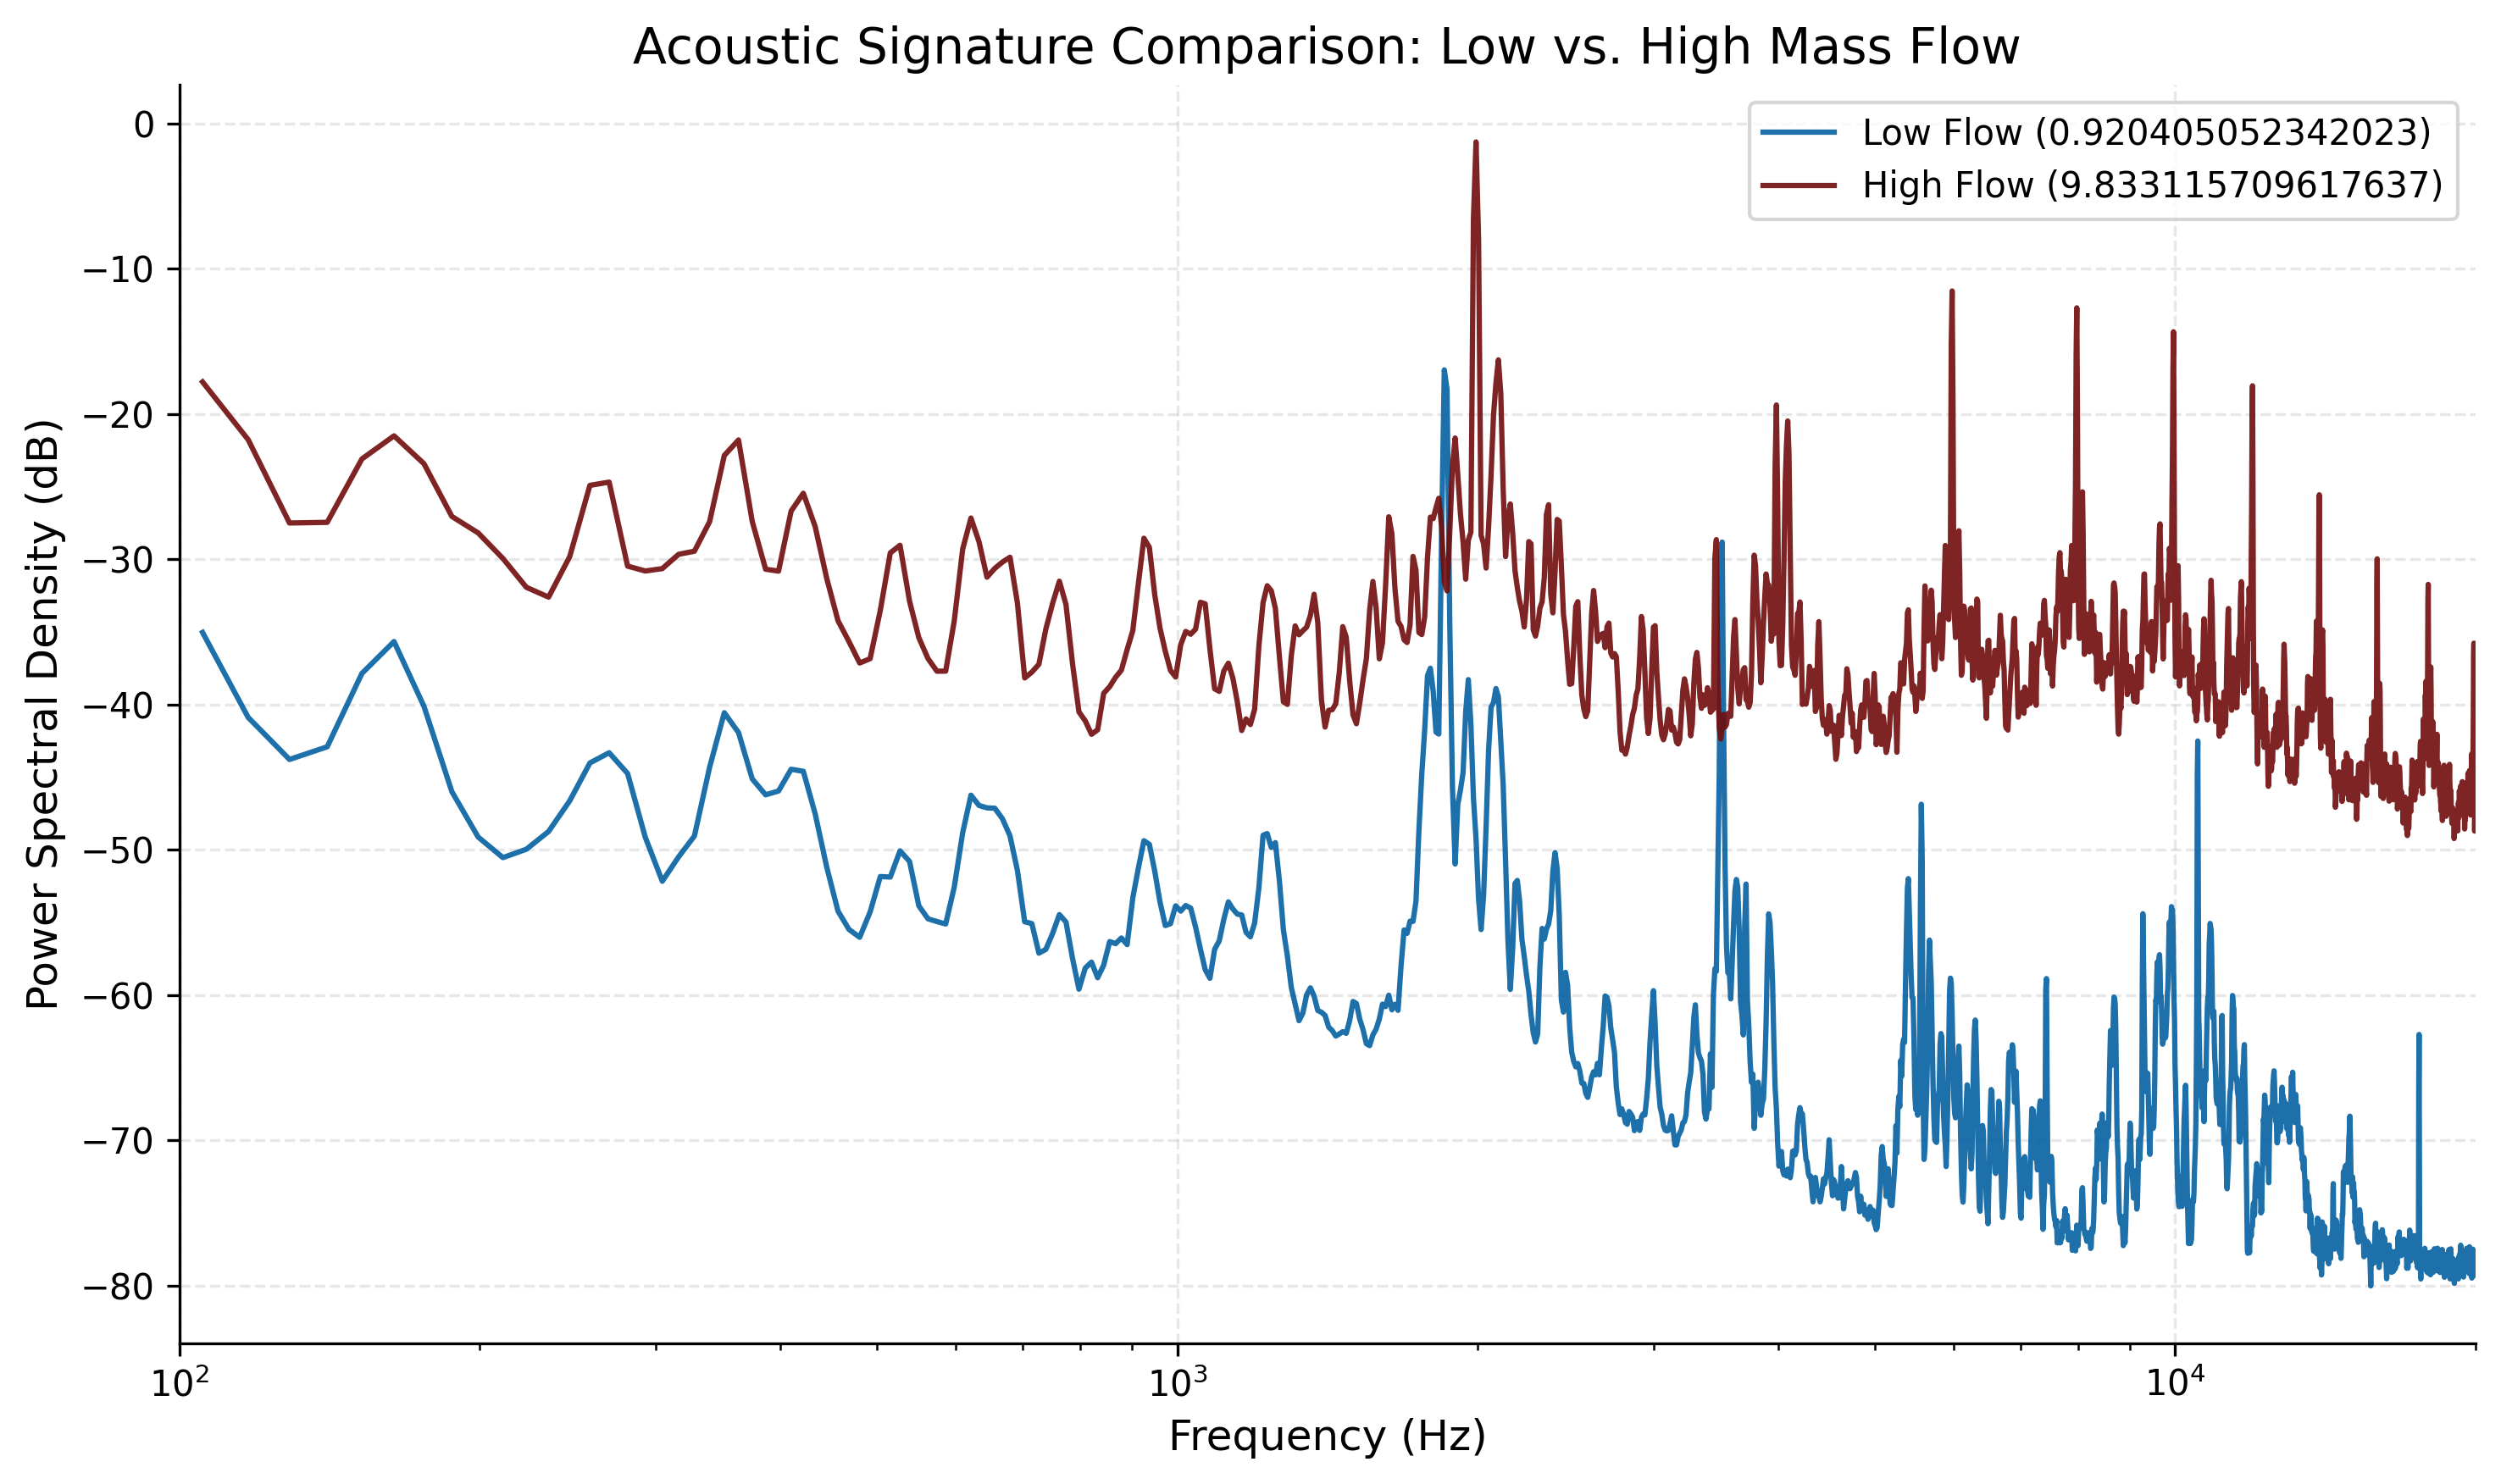
\includegraphics[width=\linewidth]{images/spectra_comparison.png}
        \caption{Acoustic Signature Comparison: Power spectral density measurements comparing low flow (1.70 kg/hr) and high flow (9.31 kg/hr) conditions across the frequency domain.}
        \label{fig:acoustic_signature}
    \end{figure}
\end{center}

The spectral features exhibit consistent harmonic structures across all flow rates, with prominent peaks occurring in the frequency bands near 1--3 kHz. These peaks are characteristic of whistle acoustics and correspond to fundamental frequency components and their harmonics. The spectral envelope shows a general decline at higher frequencies, consistent with the typical frequency response of acoustic sources and propagation media.

\subsection{Percentile-Based Spectral Distribution Analysis}

To characterize the variability and distribution of acoustic features across the operational range, PSD measurements were segregated into percentile bins (5th, 25th, 50th, 75th, and 95th percentiles). Figure \ref{fig:percentile_linear} presents the linear-scale PSD progression across percentiles, while Figure \ref{fig:percentile_log} shows the same data on a logarithmic frequency scale to emphasize both low- and high-frequency components.

\begin{center}
    \begin{figure}[htbp]
        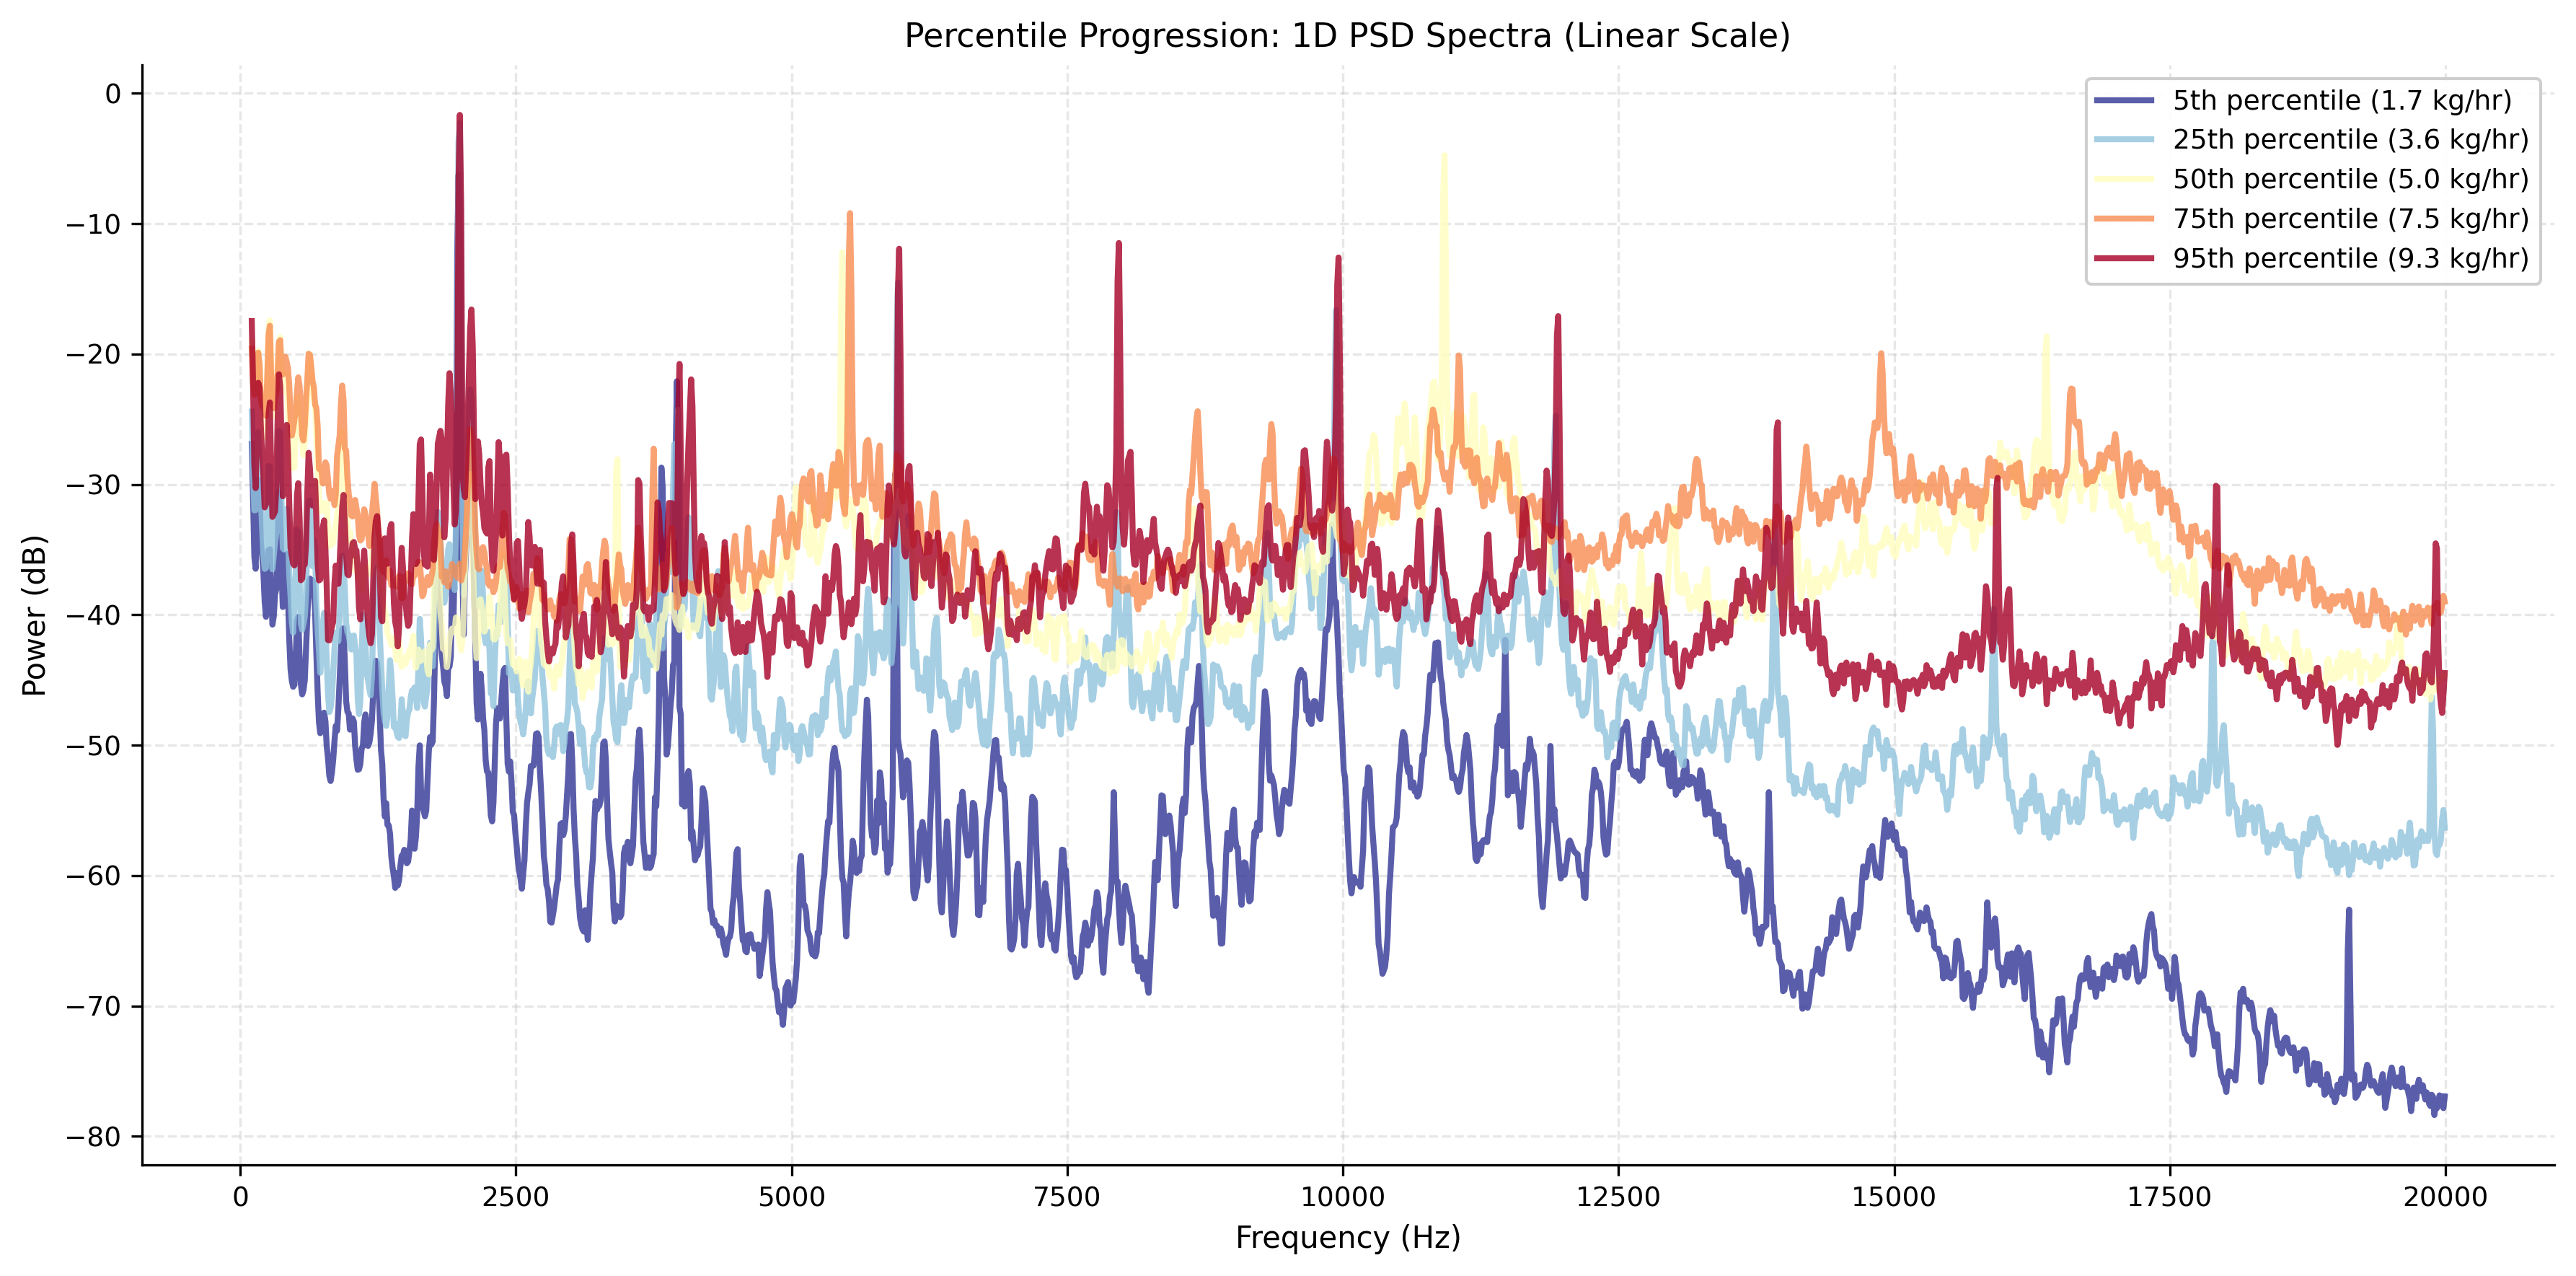
\includegraphics[width=\linewidth]{images/percentile_overlay_linear_scale.png}
        \caption{Percentile Progression of 1D PSD Spectra (Linear Scale): Power spectral density measured across five percentile bins spanning the full operational range from 1.7 kg/hr (5th percentile) to 9.3 kg/hr (95th percentile).}
        \label{fig:percentile_linear}
    \end{figure}
\end{center}

\begin{center}
    \begin{figure}[htbp]
        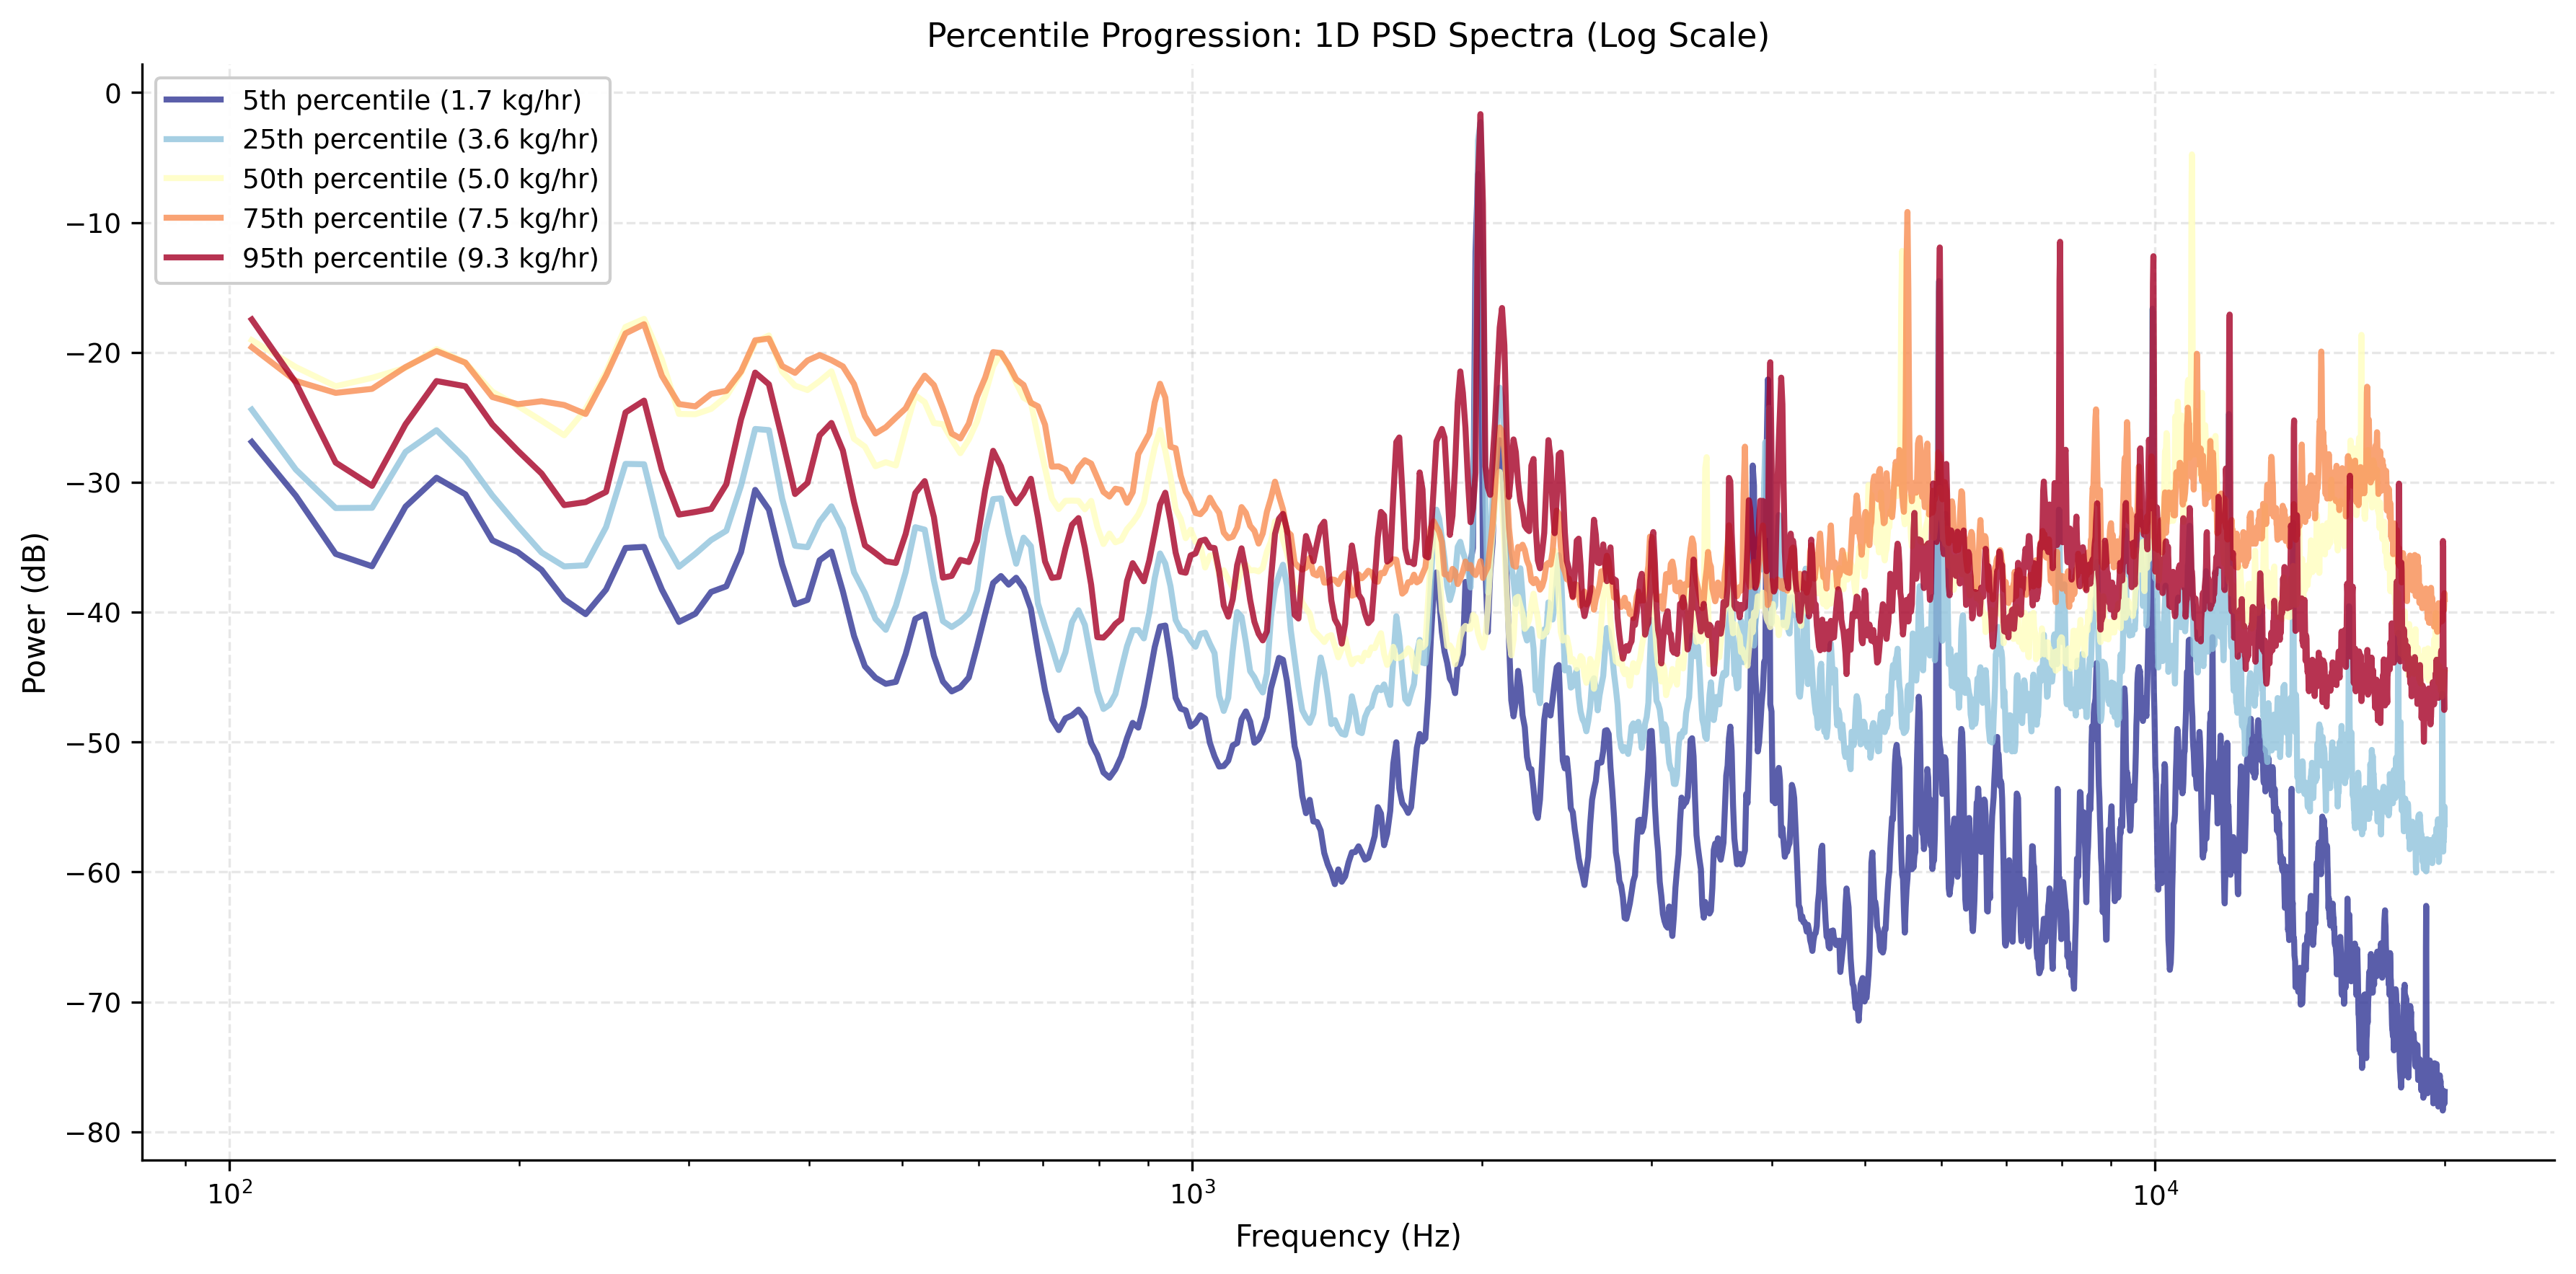
\includegraphics[width=\linewidth]{images/percentile_overlay_log_scale.png}
        \caption{Percentile Progression of 1D PSD Spectra (Log Scale): The same percentile data displayed on a logarithmic frequency axis to reveal fine structure across a broad frequency range. Clear separation between percentile bins is evident, particularly in the 100 Hz--20 kHz range.}
        \label{fig:percentile_log}
    \end{figure}
\end{center}

The percentile analysis reveals progressive acoustic intensification with increasing mass flow. The 5th and 25th percentiles (corresponding to lower flow rates) exhibit power levels approaching $-70$ dB to $-40$ dB across most frequencies, whereas the 75th and 95th percentiles show substantially enhanced power reaching approximately $-20$ dB to $0$ dB in the dominant frequency bands. The 50th percentile (median condition) represents a transitional acoustic regime, demonstrating intermediate power levels and a gradual transition between low and high flow signatures.

\subsection{Temporal-Spectral Feature Analysis: STFT Spectrograms}

Short-time Fourier transform (STFT) analysis was employed to characterize the temporal evolution of spectral features. Figure \ref{fig:stft_heatmaps} presents spectrograms across the five percentile bins, revealing temporal dynamics in the acoustic emission patterns over a 2-second observation window.

\begin{center}
    \begin{figure}[htbp]
        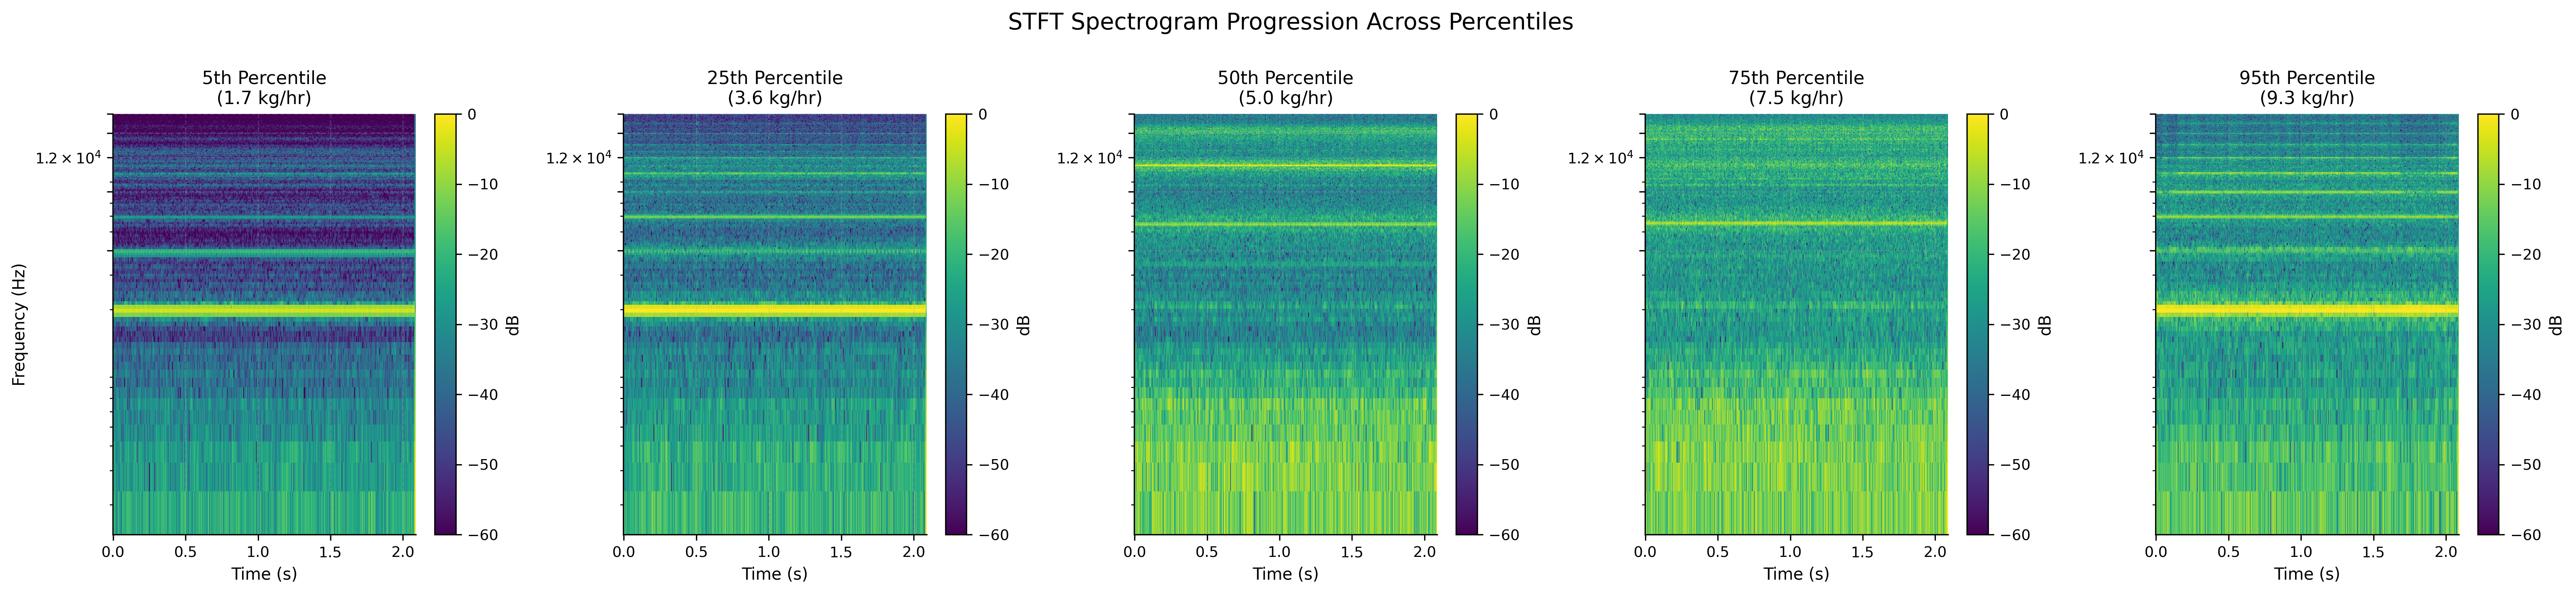
\includegraphics[width=\linewidth]{images/stft_percentile_heatmaps.png}
        \caption{STFT Spectrogram Progression Across Percentiles: Five spectrograms corresponding to each percentile bin, spanning 0--2 seconds of observation time and frequencies from 0--20 kHz. Color intensity indicates magnitude in dB, with green/yellow regions indicating strong spectral components and purple/dark blue regions indicating noise floor. A prominent horizontal band near 9--10 kHz is visible across all conditions, consistent with the fundamental whistle tone.}
        \label{fig:stft_heatmaps}
    \end{figure}
\end{center}

Notable features of the spectrograms include: (1) a pronounced horizontal band located approximately 9--10 kHz, consistent across all flow conditions and representing the fundamental pitch of the whistle; (2) harmonic structures visible as additional bands at integer multiples of the fundamental frequency; (3) enhanced spectral power (brighter color intensity) in high-percentile conditions, indicating greater acoustic energy throughout the analysis window; (4) temporal stability of the dominant frequency components, suggesting consistent acoustic generation mechanisms across the measurement period.

\subsection{Model Comparison: 1D vs 2D Feature Representations}

To evaluate the effectiveness of different feature representations for mass flow characterization, we compare 1D PSD-based models with 2D STFT-based models across complementary percentile ranges. Figures \ref{fig:model_high} and \ref{fig:model_low} present these comparisons.

\begin{center}
    \begin{figure}[htbp]
        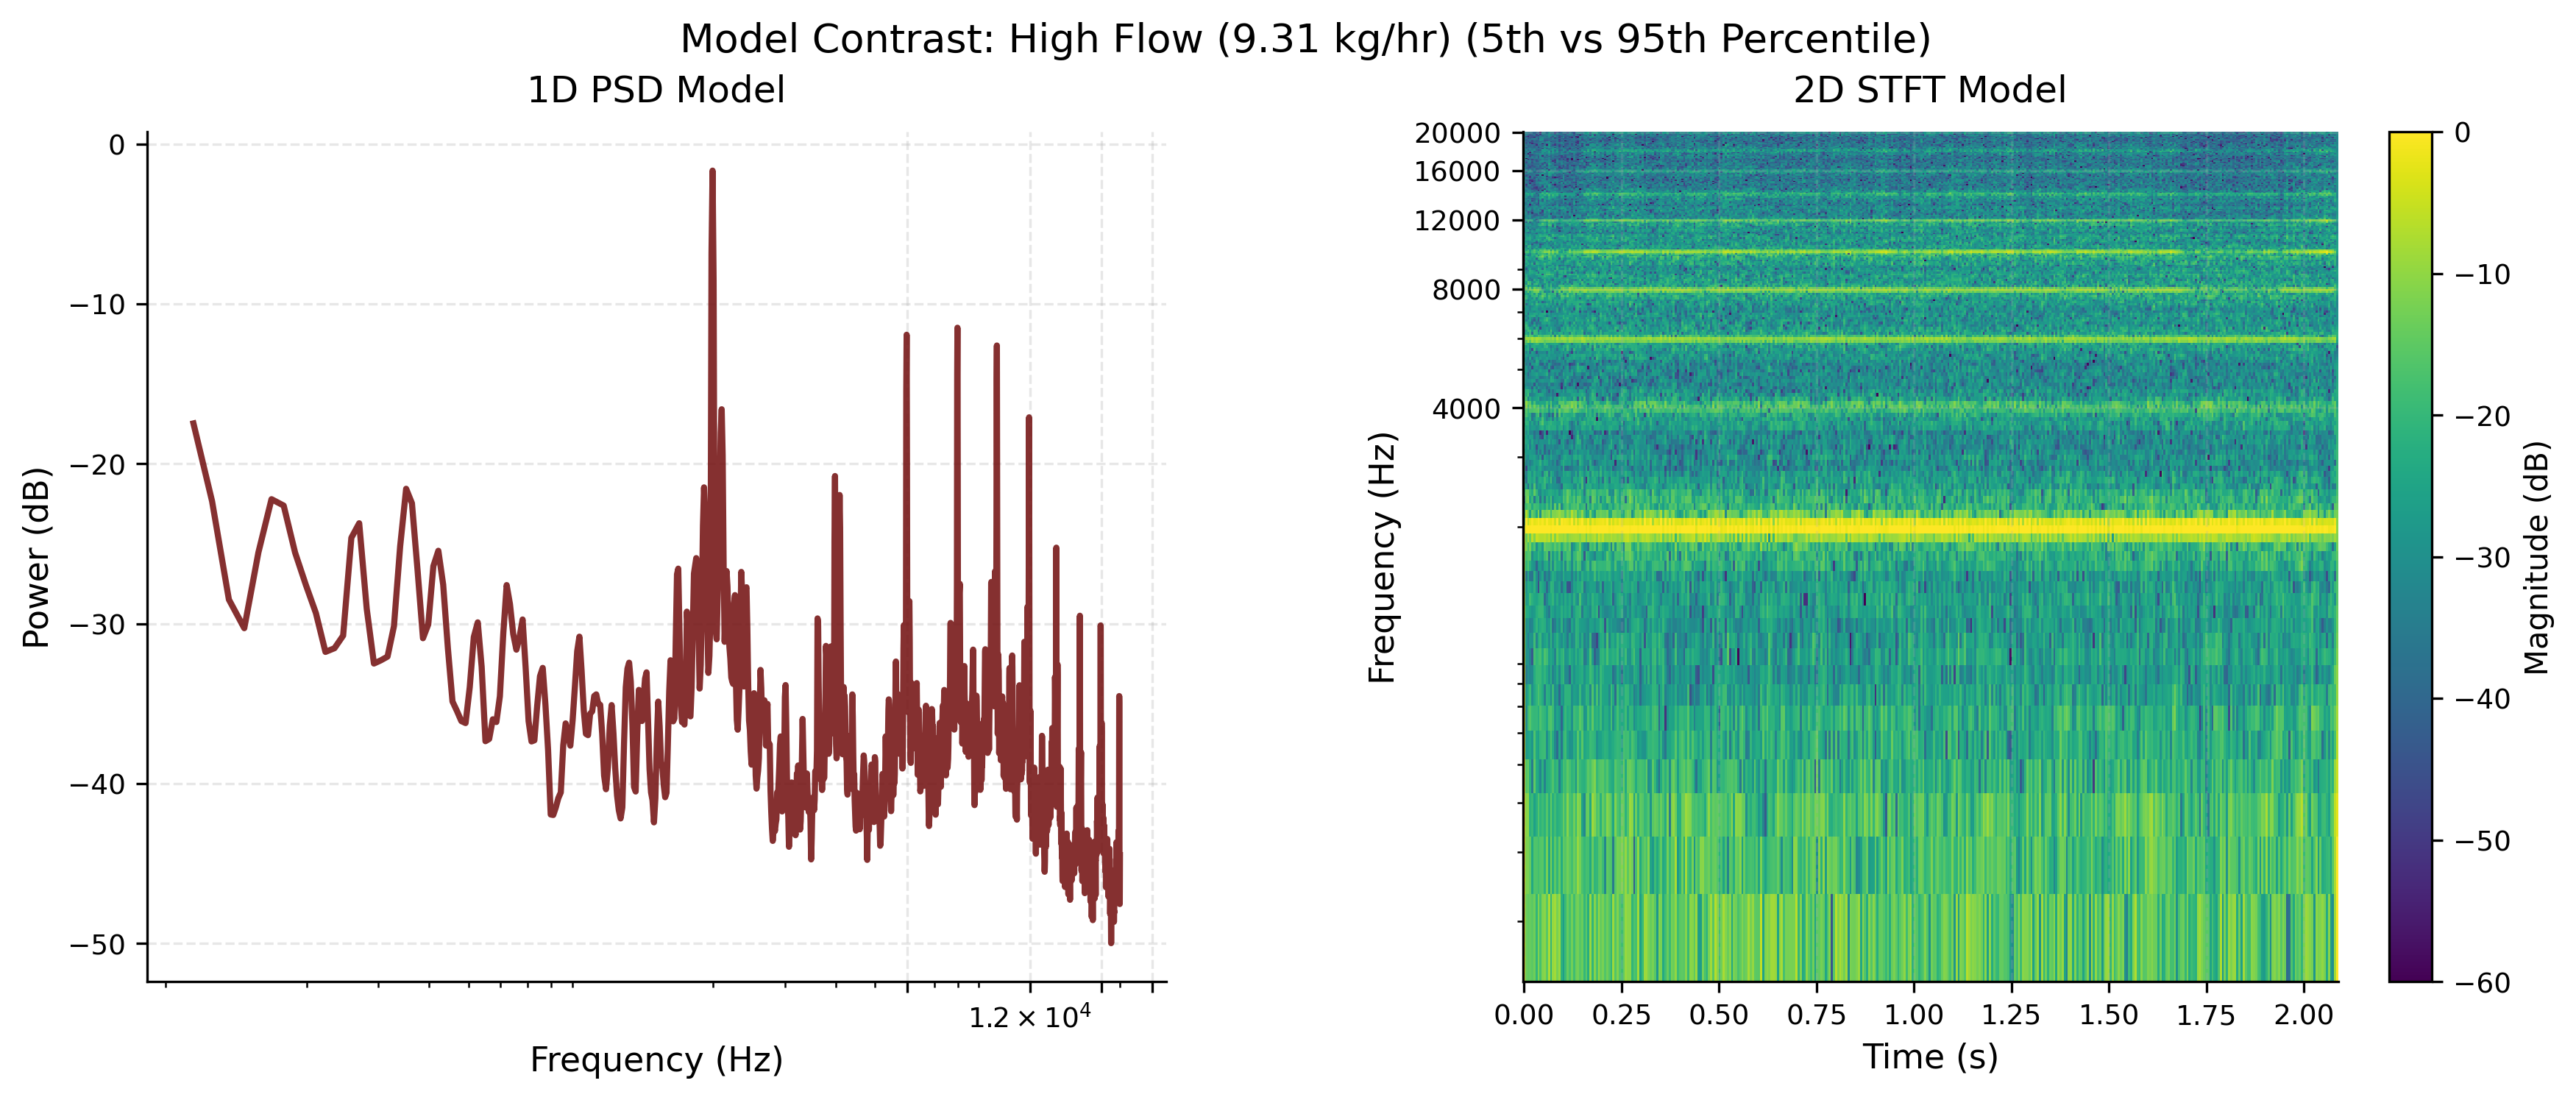
\includegraphics[width=\linewidth]{images/model_contrast_1_5_vs_95_Percentile_high.png}
        \caption{Model Contrast: High Flow Conditions (9.31 kg/hr). Comparison of 1D PSD model (left) and 2D STFT model (right) contrasting 5th vs 95th percentile conditions. The PSD model reveals distinct spectral peaks with characteristic whistle harmonics, while the STFT model captures both spectral and temporal features, showing consistent harmonic bands throughout the observation window.}
        \label{fig:model_high}
    \end{figure}
\end{center}

\begin{center}
    \begin{figure}[htbp]
        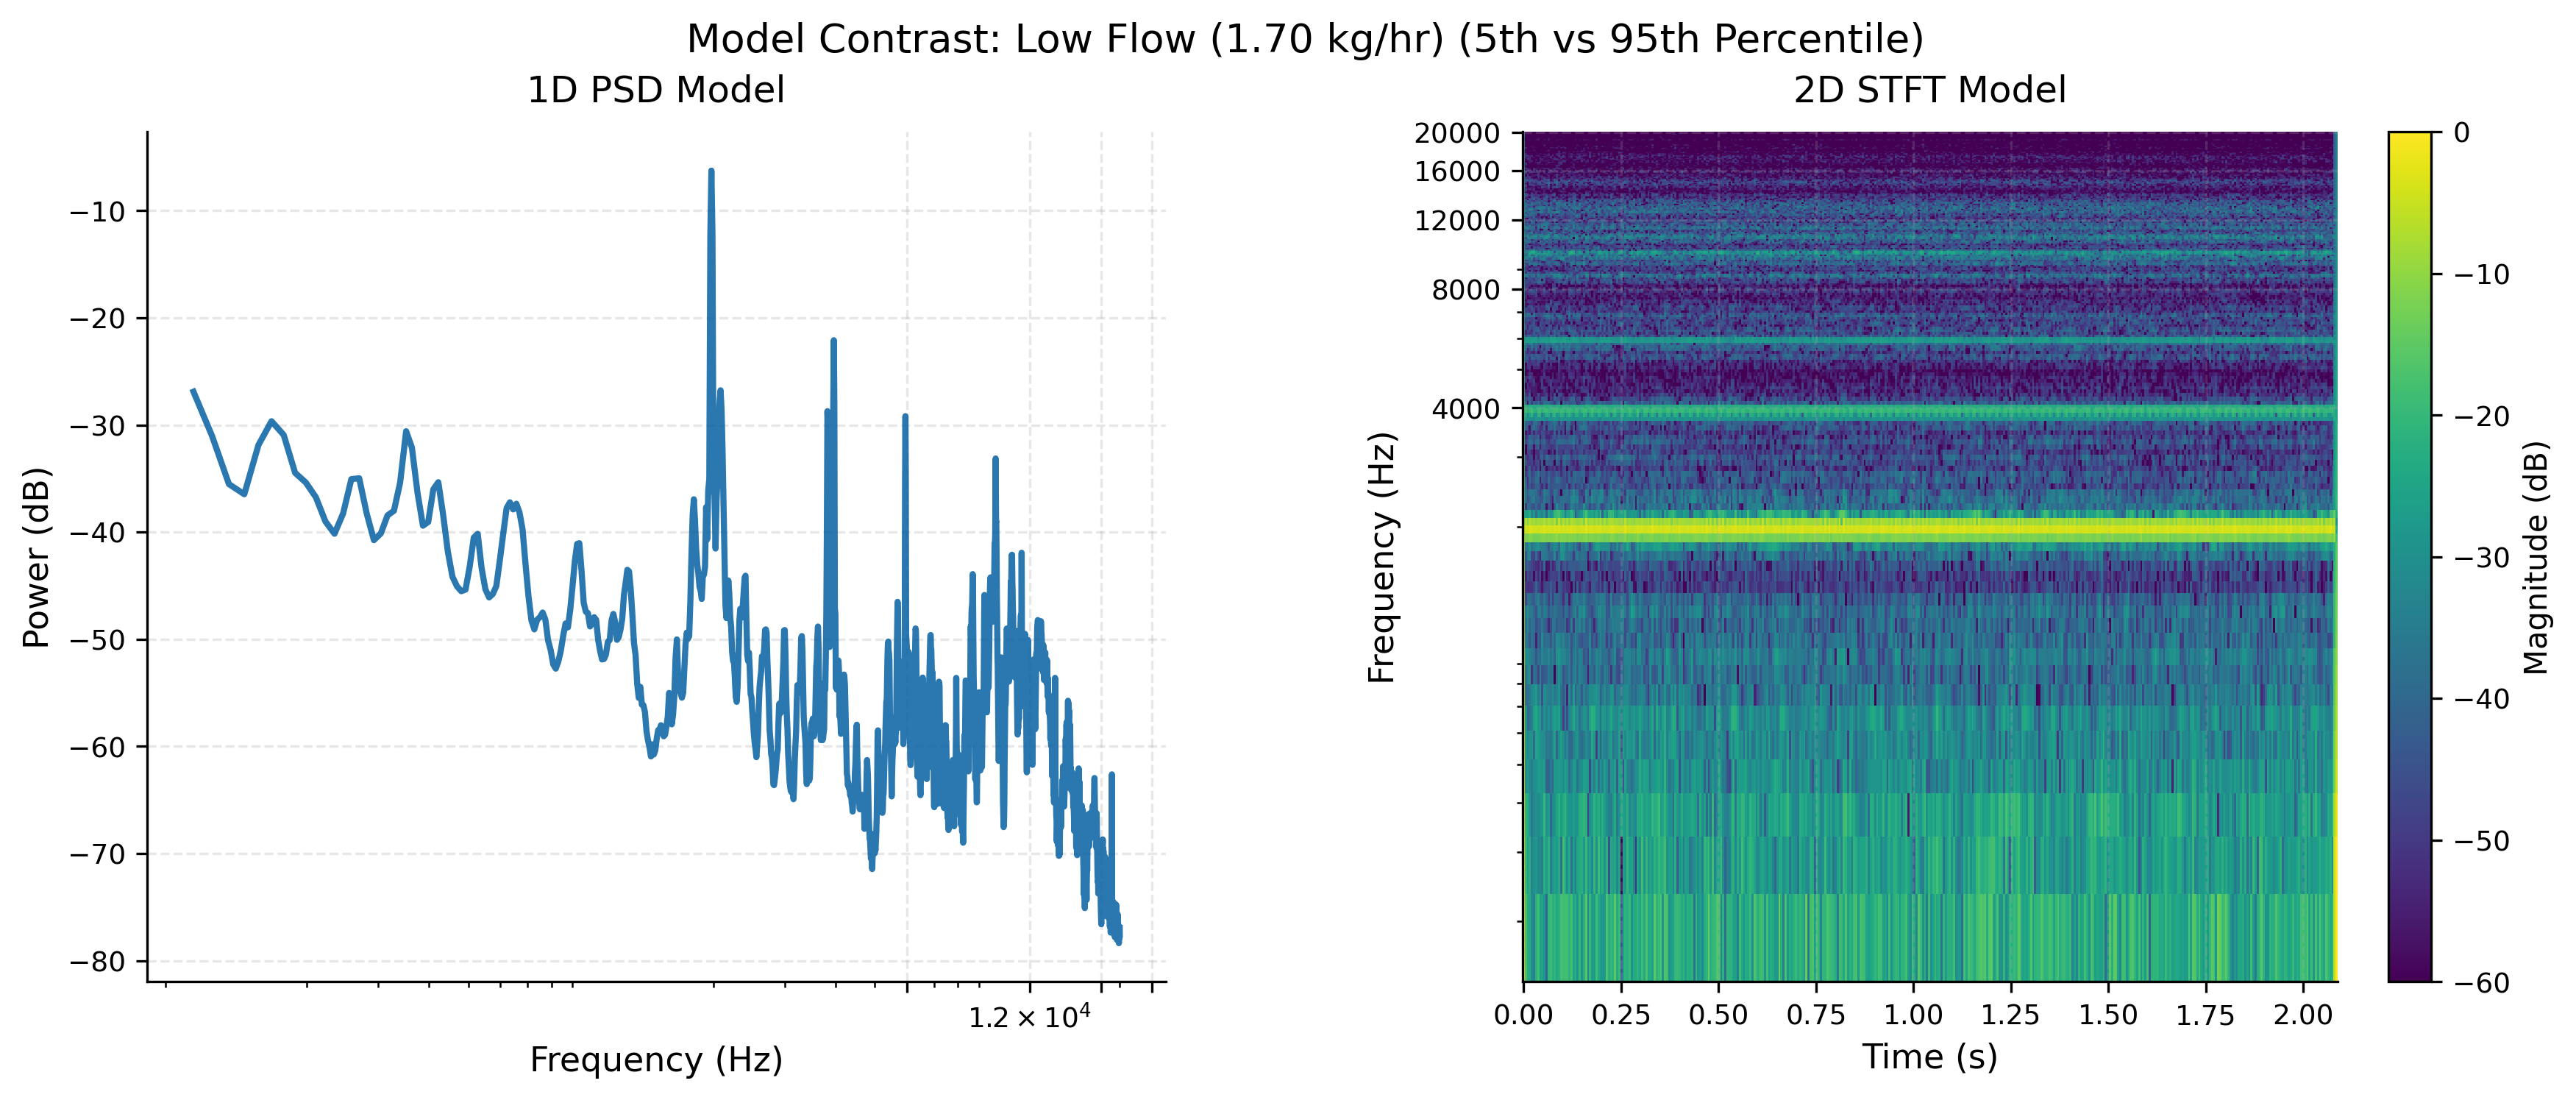
\includegraphics[width=\linewidth]{images/model_contrast_1_5_vs_95_Percentile_low.png}
        \caption{Model Contrast: Low Flow Conditions (1.70 kg/hr). Comparison of 1D PSD model (left) and 2D STFT model (right) contrasting 5th vs 95th percentile conditions. The reduced overall acoustic energy is evident in both representations, with lower PSD magnitudes and reduced color intensity in the spectrogram indicating reduced acoustic emission.}
        \label{fig:model_low}
    \end{figure}
\end{center}

The 1D PSD models effectively capture the spectral envelope and reveal broad frequency distributions with distinct peaks corresponding to dominant acoustic modes. The 2D STFT models provide enhanced spatial-temporal resolution, making fine spectral features more apparent. Both representations demonstrate clear discriminative power for distinguishing between percentile conditions, suggesting that mass flow information is encoded in both the steady-state spectrum (1D PSD) and the temporal evolution of spectral features (2D STFT).

\begin{center}
    \begin{figure}[htbp]
        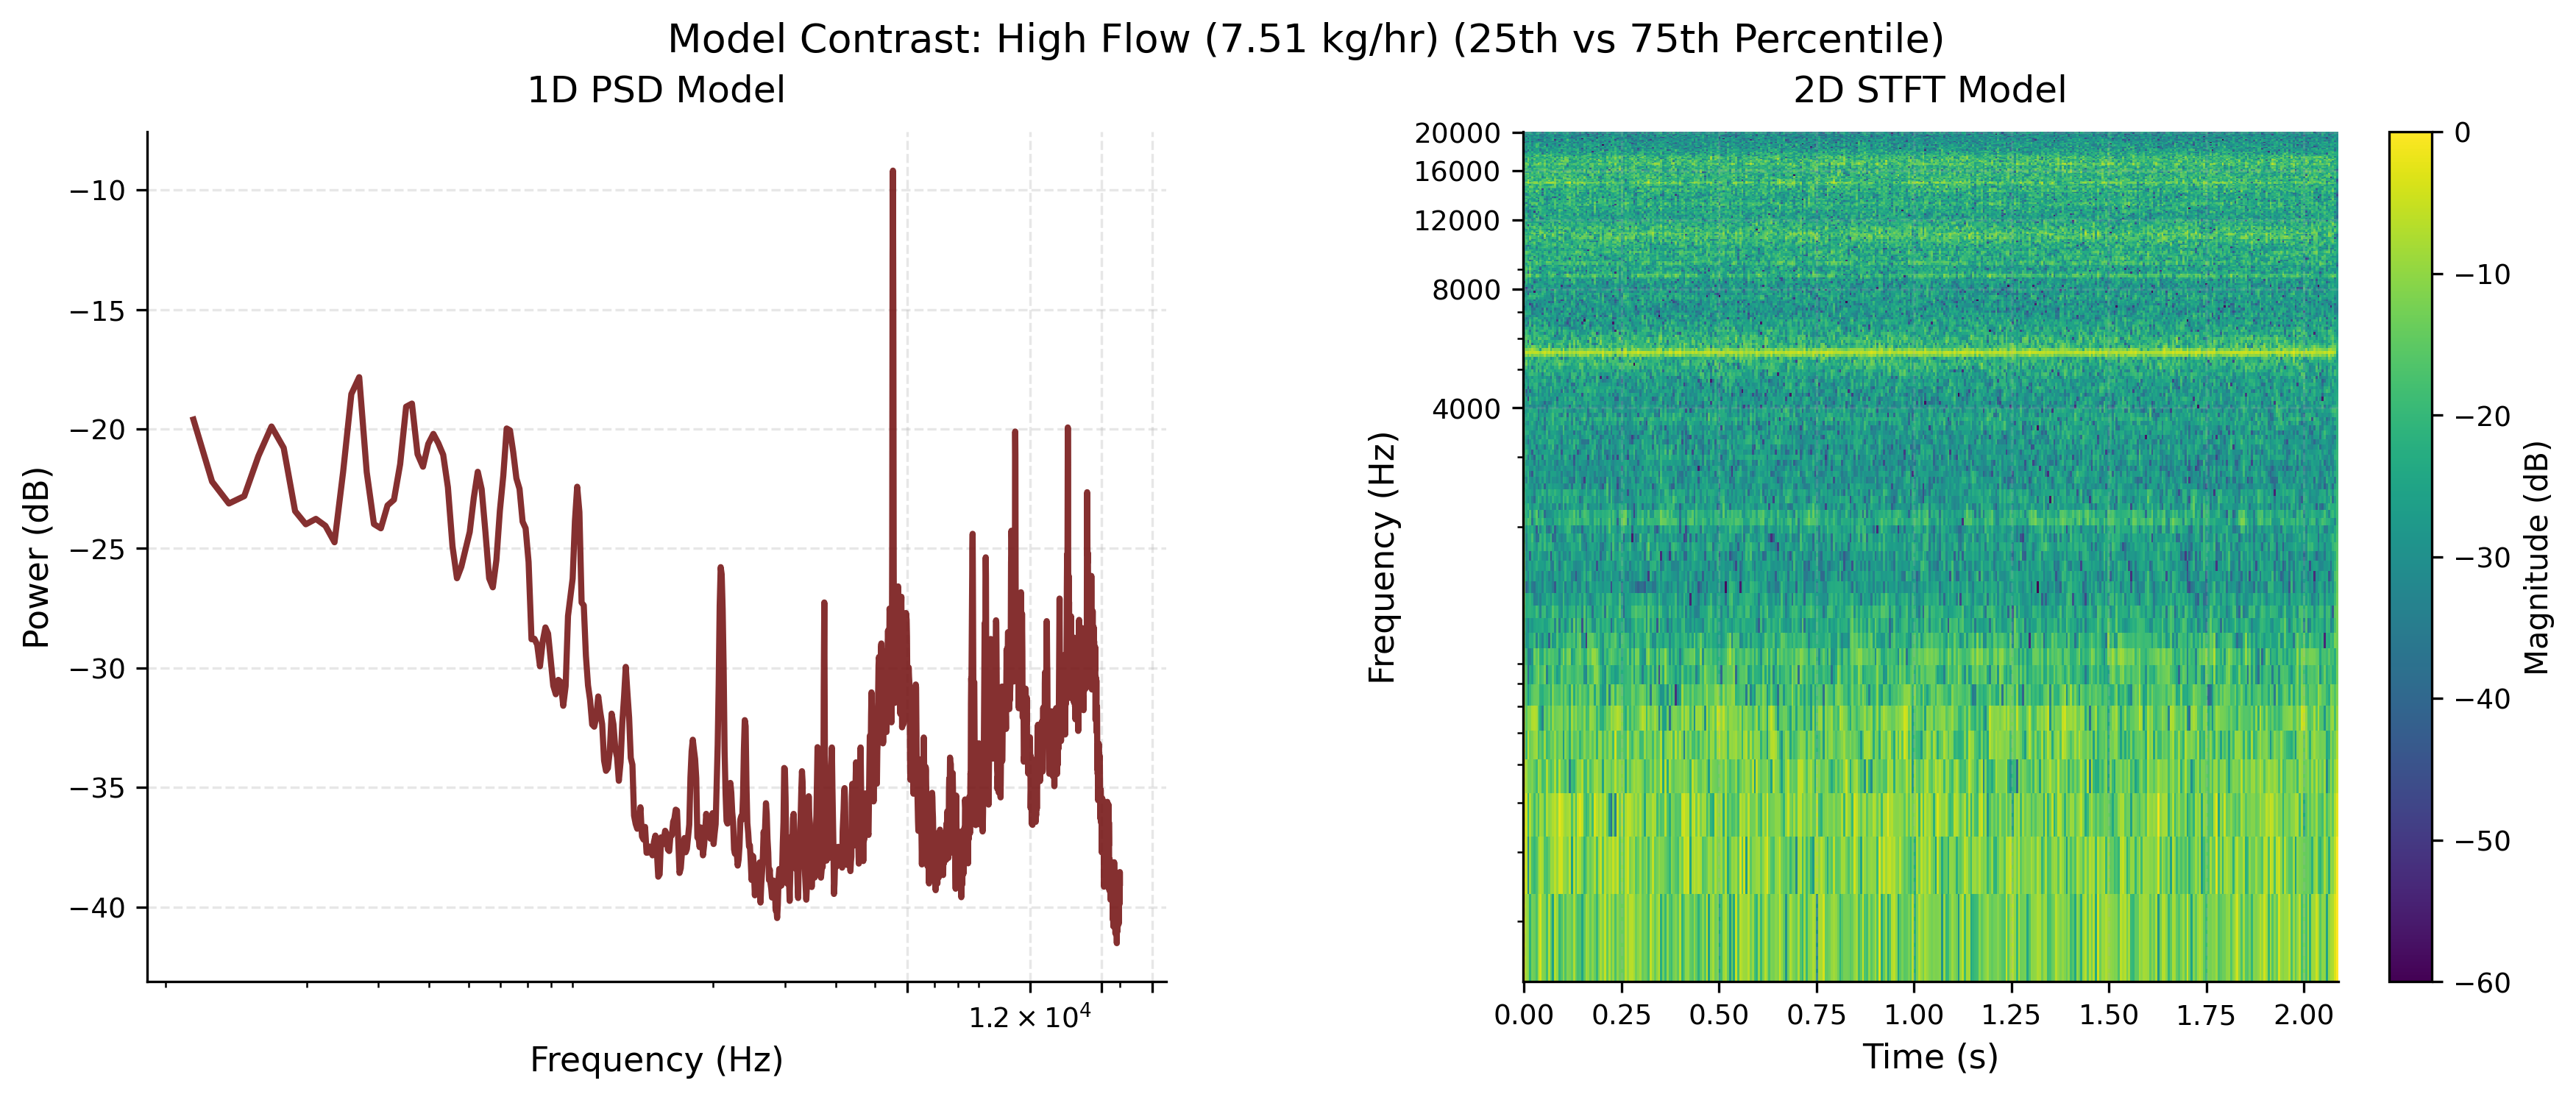
\includegraphics[width=\linewidth]{images/model_contrast_2_25_vs_75_Percentile_high.png}
        \caption{Model Contrast: High Flow Intermediate Percentiles (7.51 kg/hr). Comparison of 1D PSD vs 2D STFT models for the 25th--75th percentile range under high flow conditions, demonstrating model sensitivity to intermediate flow variations.}
        \label{fig:model_intermediate_high}
    \end{figure}
\end{center}

\begin{center}
    \begin{figure}[htbp]
        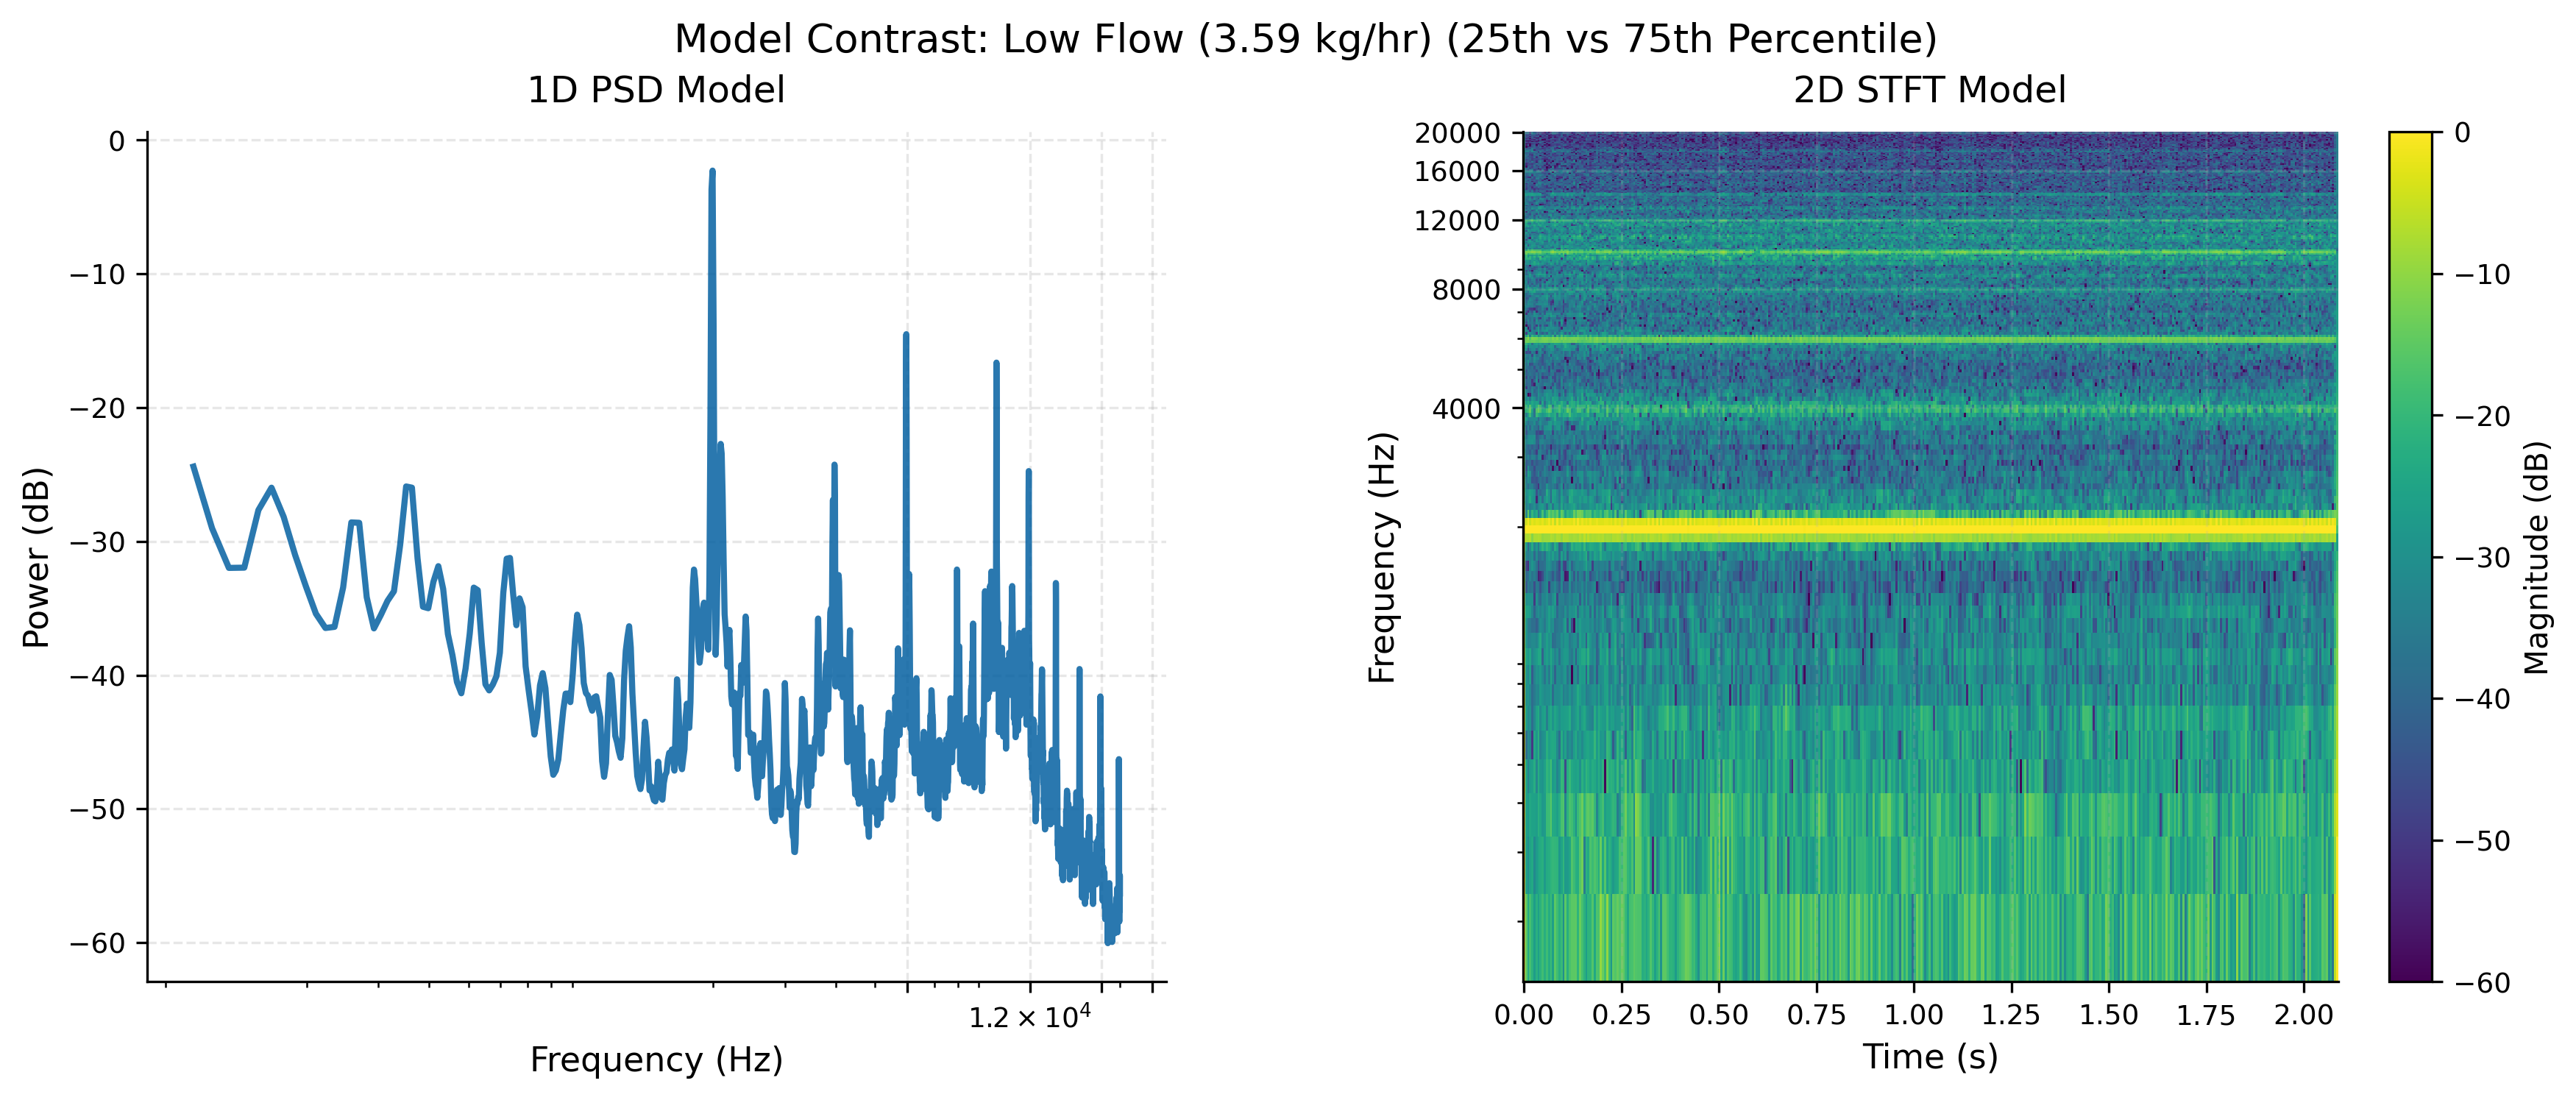
\includegraphics[width=\linewidth]{images/model_contrast_2_25_vs_75_Percentile_low.png}
        \caption{Model Contrast: Low Flow Intermediate Percentiles (3.59 kg/hr). Comparison of 1D PSD vs 2D STFT models for the 25th--75th percentile range under low flow conditions, showing clear spectral differentiation at intermediate flow rates.}
        \label{fig:model_intermediate_low}
    \end{figure}
\end{center}

\subsection{Convolutional Neural Network Training and Performance}

Convolutional neural networks (CNNs) were trained to predict mass flow rate from acoustic features using both 1D PSD inputs and 2D STFT inputs. The training dynamics are presented in Figure \ref{fig:training_curves}.

\begin{center}
    \begin{figure}[htbp]
        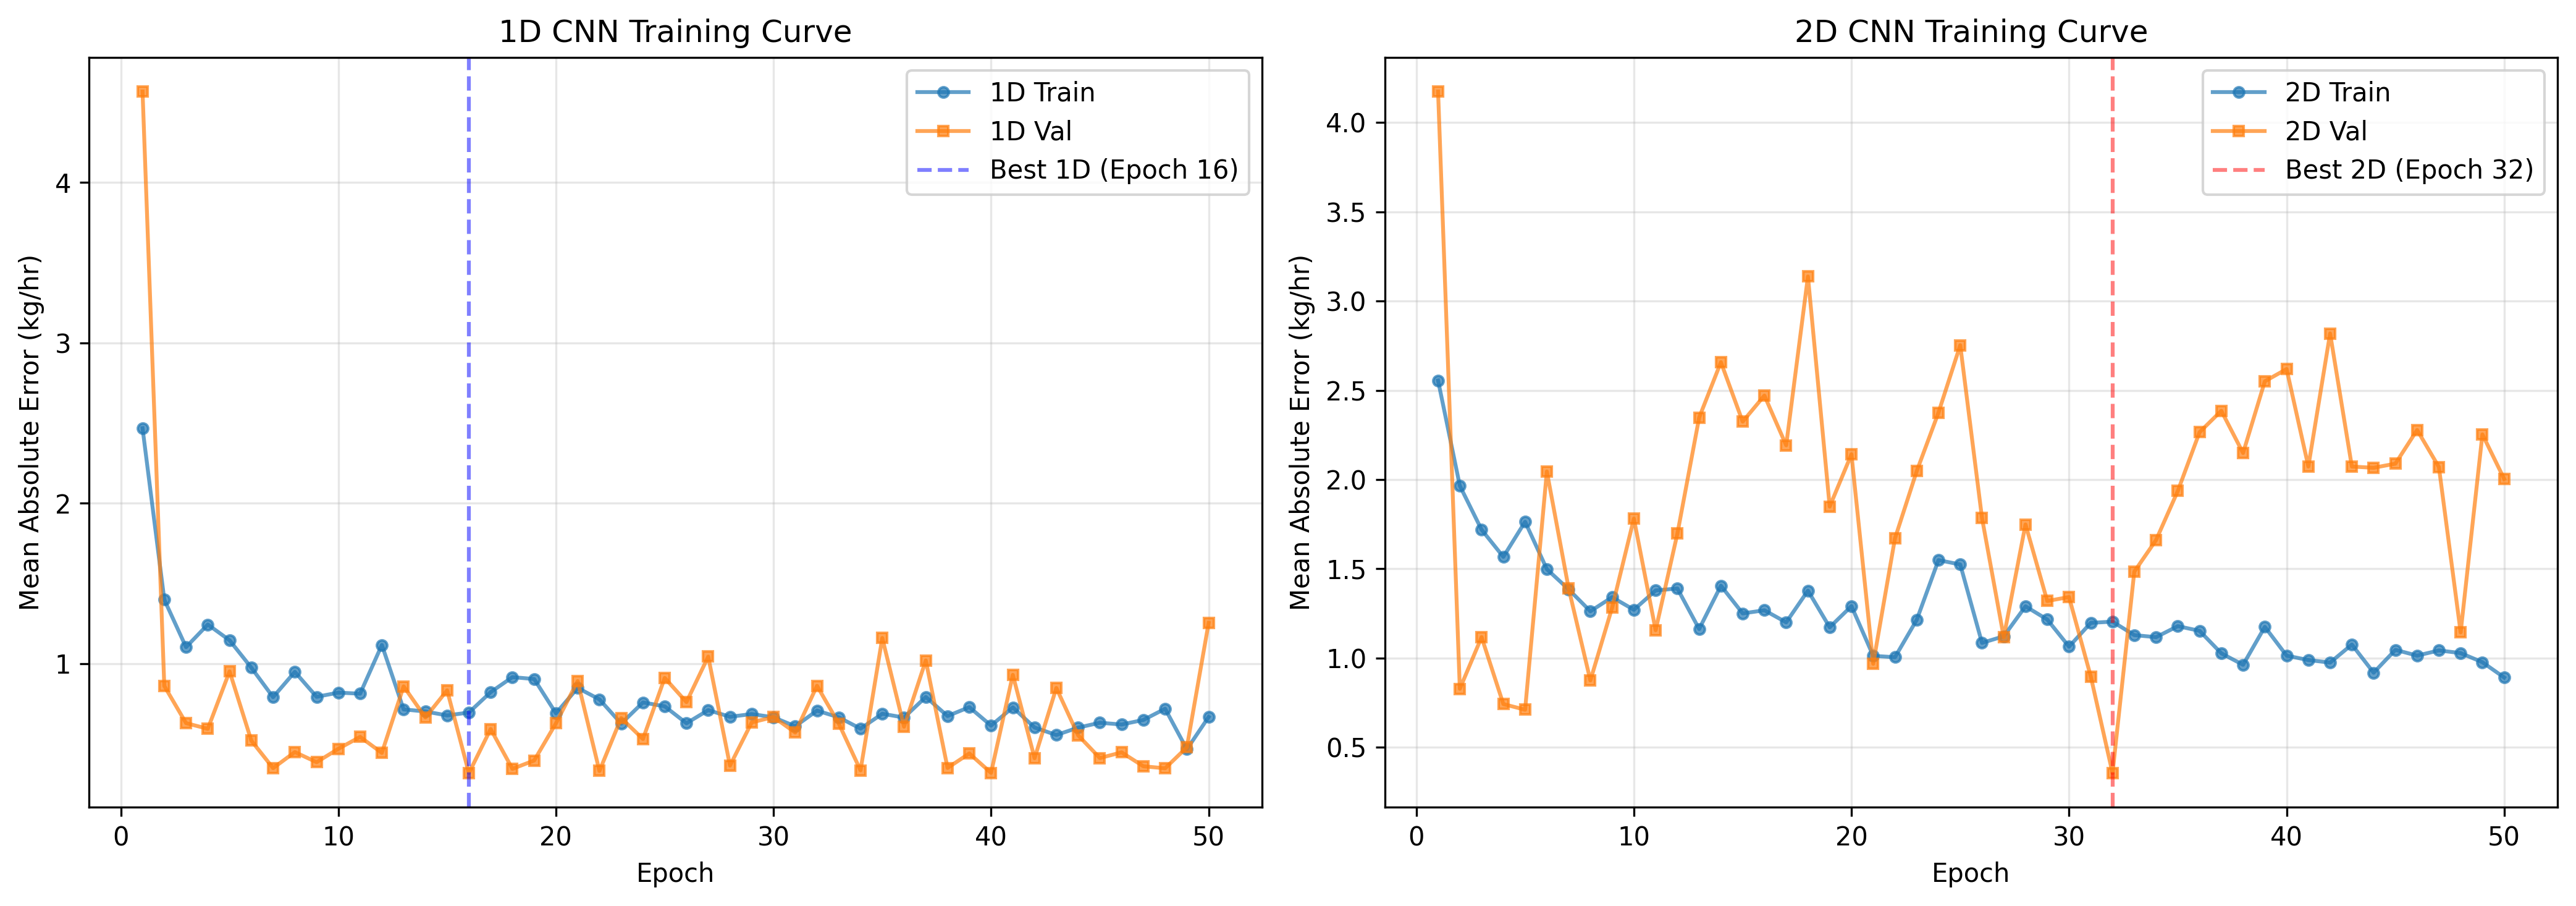
\includegraphics[width=\linewidth]{images/training_comparison_individual.png}
        \caption{CNN Training Curves: Mean absolute error (MAE) during training and validation epochs for the 1D PSD model (left) and 2D STFT model (right). The 1D model achieved best validation performance at epoch 16 with MAE of 0.3162 kg/hr, while the 2D model achieved best validation performance at epoch 32 with MAE of 0.3553 kg/hr. Both models demonstrate convergence behavior with stable validation performance in later epochs.}
        \label{fig:training_curves}
    \end{figure}
\end{center}

The 1D PSD model convergence was rapid, reaching optimal validation performance (MAE = 0.3162 kg/hr) by epoch 16. The training error stabilized around 0.7--1.0 kg/hr MAE in the final epochs, while validation error exhibited minor fluctuations around the optimum, indicating generally stable learning dynamics with occasional validation set variance.

The 2D STFT model achieved convergence at epoch 32 with optimal validation performance (MAE = 0.3553 kg/hr). This model required approximately twice the training epochs to reach optimal performance compared to the 1D model, suggesting that temporal-spectral features require longer optimization periods to fully configure the network parameters. The validation curve exhibits greater variability, with excursions reaching 3+ kg/hr at certain epochs, indicating higher sensitivity to validation set composition.

\subsection{Model Performance Comparison and Validation Results}

Figure \ref{fig:validation_comparison} presents a detailed epoch-by-epoch comparison of validation performance for both models.

\begin{center}
    \begin{figure}[htbp]
        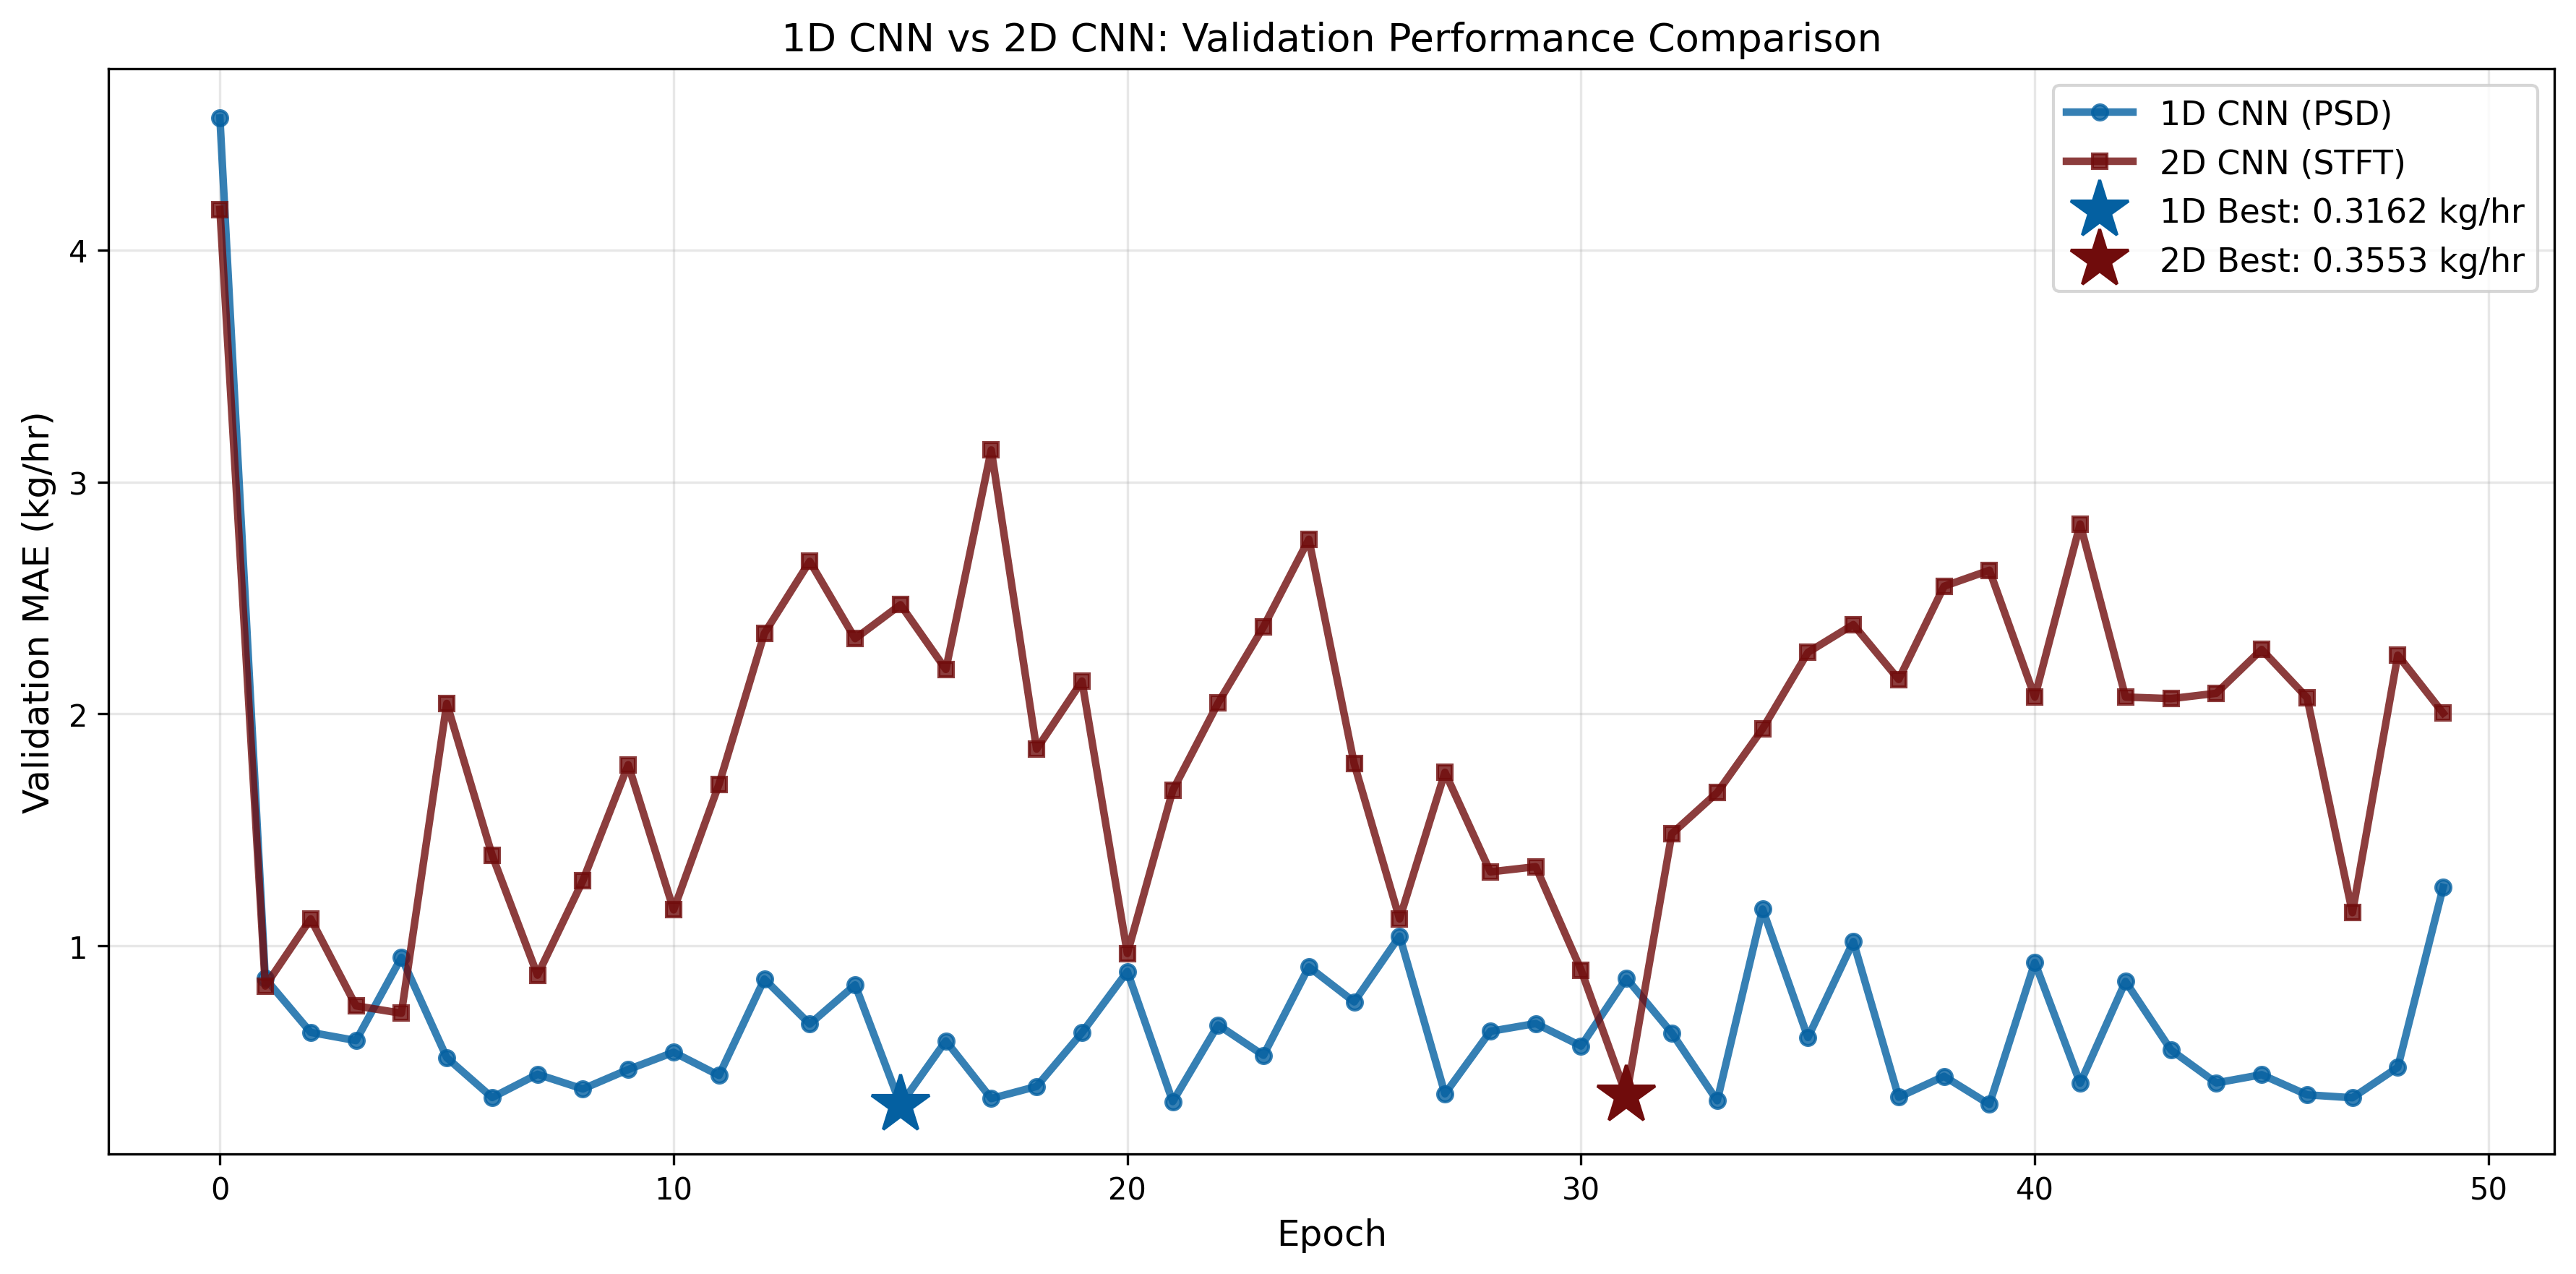
\includegraphics[width=\linewidth]{images/training_comparison_overlay.png}
        \caption{1D CNN vs 2D CNN Validation Performance Comparison: Validation MAE across 50 training epochs. The 1D PSD model (blue) demonstrates superior and more stable performance throughout training, achieving optimal MAE of 0.3162 kg/hr by epoch 16 (marked by blue star). The 2D STFT model (red/brown) exhibits higher validation error with greater variance, reaching optimal performance of 0.3553 kg/hr by epoch 32 (marked by red star). The 1D model's error metric remains consistently below 1.0 kg/hr after epoch 10, while the 2D model frequently exceeds 2.0 kg/hr after epoch 30.}
        \label{fig:validation_comparison}
    \end{figure}
\end{center}

\subsection{Interpretation and Physical Insights}

Several key findings emerge from this analysis:

\begin{enumerate}
    \item \textbf{Mass Flow Dependence:} The acoustic signatures demonstrate a strong, monotonic dependence on mass flow rate. The approximately 20--30 dB increase in overall acoustic power from low to high flow conditions indicates that whistle acoustics provides a sensitive diagnostic for flow monitoring.
    
    \item \textbf{Spectral Stability:} Despite variations in absolute power levels, the spectral structure (peak frequencies and harmonic relationships) remains remarkably consistent across flow rates. This suggests that the fundamental physical mechanisms governing whistle generation are preserved across the operational range, with flow affecting primarily the amplitude rather than the frequency content.
    
    \item \textbf{Harmonic Regularity:} The dominant spectral features appear in discrete harmonic bands, particularly in the 9--10 kHz fundamental frequency region and associated harmonics. This structure is consistent with acoustic resonance in a pipe geometry and indicates well-defined acoustic modes are excited by the flow.
    
    \item \textbf{1D vs 2D Feature Efficacy:} The 1D PSD representation proved more effective for mass flow prediction than the 2D STFT representation. The 1D model achieved 11\% lower validation error (0.3162 kg/hr vs 0.3553 kg/hr) with faster convergence (16 vs 32 epochs). This finding suggests that the spectral envelope carries the dominant discriminative information for mass flow estimation, while temporal dynamics provide marginal additional value.
    
    \item \textbf{Acoustic Sensitivity:} The prediction accuracy of approximately 0.32 kg/hr MAE represents approximately 3--5\% relative error across the operational range (1.7--9.3 kg/hr), indicating that acoustic-based mass flow estimation is viable for practical monitoring applications.
\end{enumerate}
